\graphicspath{{./Aplikacja/images}}

\chapter{Aplikacja pulpitowa}

Aplikacja będąca obiektem tego podrozdziału stanowi rdzeń systemu kontroli, dzięki któremu oparator urządzenia jest nim w stanie sterować oraz zbierać z jego pomocą dane. Zawiera ona moduły do komunikacji ze wszystkimi częściami urządzenia, oraz zestaw wykresów aktualizowanych w czasie rzeczywistym. Pomimo względnie prostych funkcji, aplikacja posiada złożoną budowę ze względu na rówoległą obsługę różnych dróg komunikacji. Budowa ta w szczegółach opisana zostanie  w dalszej części tego rozdziału.

\section{Rola i założenia aplikacji}

Aplikacja była rozwijana mając na uwadze poniższe założenia:
\begin{itemize}
	\item Aplikacja powinna umożliwiać oparatorowi zadanie prędkości obu stopni swobody klinostatu oraz objętości wody, która ma zostać dostarczona co wskazany przez operatora interwał czasowy.
	\item Aplikacja powinna dawać dostęp do danych o orientacji komory względem wektora grawitacji, uśrednionej grawitacji i temperatury z ostatnich 60 sekund. Dane odnośnie wilgotności podłoża z uwagi na korozję czujnika przeprowadzane są znacznie rzadziej. Dodatkowo na jednym z wykresów przedstawiana ma być transformata Fouriera sygnału uzyskanego z akcelerometru.
	\item Aplikacja powinna posiadać podstawowe zabezpieczenia, aby uniemożliwić operatorowi zawieszenie urządzenia poprzez nieświadome wykonanie operacji niedozwolonych. Powinny również znaleźć się w niej zabezpieczenia obsługujące błędy generowane przez fizyczne odłączenie klinostatu w momencie gdy program zakłada iż jest on podłączony.
	\item Aplikacja powinna w tle posiadać uruchomiony moduł komunikacji bezprzewodowej z komorą środowiskową. Połączenie to służyć ma wymianie danych oraz nastawie intensywności oświetlenia.
	\item Oprator powinien mieć możliwość zapisania zebranych wyników pomiarów do pliku .csv.
	\item Powinien istnieć podstawowy system komunikatów, który będzie informować operatora o rezultatach jego operacji.
\end{itemize}

\section{Wybrany język i biblioteki}

W celu implementacji aplikacji wybrany został język Python. Wybór ten motywowany był moją dobrą znajomością tego języka, oraz poprzednim doświadczeniem w tworzeniu aplikacji z graficznym interfejsem użytkownika w tym języku. Interfejs został stworzony z użyciem biblioteki \textbf{Tkinter}, która oferuje względnie proste tworzenie takich aplikacji w konwencji programowania obiektowego, z której to intensywnie korzystano podczas rozwoju programu. Do realizacji łącza bezprzewodowego z komorą środowiskową wykorzystano bibliotekę \textbf{socket}, pozwalającą na utworzenie takiego łącza w lokalnej sieci poprzez protokół TCP (ang. \angver{Transmission Control Protocl}). Do działania programu niezbędna okazała się biblioteka \textbf{threading}, pozwalająca na współbieżne wykonywanie różnych jego części. Transformacja Fouriera liczona jest 15 razy na sekundę z użyciem biblioteki \textbf{scipy}, a obliczenia te są zrównoleglone za pomocą biblioteki \textbf{multiprocessing} w celu ich przyspieszenia. Wykresy tworzone są wykorzystując popularną bibliotekę \textbf{matplotlib}. Oprócz tego wykorzystano również wiele innych modułów takich jak \textbf{pyserial}, \textbf{yaml}, \textbf{queue} czy \textbf{numpy} w różnych mniej znaczących celach.

\section{Podział programu na wątki}

Cała aplikacja składa się w jednym momencie z trzech rodzajów wątków:
\begin{itemize}
	\item Wątku głównego - odpowiedzialny za działanie całej aplikacji oraz tworzenie wykresów.
	\item Wątku serwera TCP - odpowiedzialny za obsługę przychodzących pakietów danych przez websocket oraz wysyłanie odpowiedzi.
	\item Wątków obsługi portu szeregowego - tworzony jedynie tymczasowo w momencie gdy należy wysłać i/lub odebrać komendę przez magistralę USB z klinostatem.
\end{itemize}
Docelowo wątek główny miał być odpowiedzialny wyłącznie za uruchamianie innych wątków oraz działanie aplikacji, natomiast tworzenie i akutualizacja wykresów miała być rezultatem działania innego, dodatkowego wątku. Takie rozwiązanie okazało się niemożliwe, ze względu na konstrukcję biblioteki matplotlib, która uniemożliwia tworzenie wykresów przez wątki inne niż główny. Związane jest to z tym iż biblioteka ta nie została stworzona w konwencji \angver{threadsafe} - bezpiecznej w działaniach między wątkami. Przy programowaniu wielowątkowym należy zwracać uwagę na występowanie tzw. wyścigów (ang. \angver{race condition}), które występują w momencie gdy przynajmniej dwa, różne wątki próbują uzyskać dostęp do tej samej, dzielonej zmiennej. Występowanie takich wyścigów jest znane w bibliotece matplotlib, a więc wykorzystywana może być ona wyłącznie w obrębie wątku głównego. Rozwiązaniem problemu wyścigów jest wykorzystanie różnego rodzaju struktur synchronizacyjnych takich jak semafory czy zamki, które zapobiegają ich występowaniu. Z tego rodzaju struktur korzysta również aplikacja.

Wątek serwera TCP jest uruchamiany przez użytkownika za pomocą odpowiedniego przycisku. Pozostaje on uruchomiony w tle aż do momentu, w którym operator postanowi zakończyć komunikację. Jego rolą jest odbieranie danych pomiarowych wysłanych z komputera komory środowiskowej oraz odesłanie odpowiedzi zawierającej informacje o obecnie ustawionym poziomie oświetlenia. Ze względu na to iż dane te muszą zostać przekazane do wątku głównego, wymiana ta zachodzi poprzez wykorzystanie struktur \textbf{Queue} z biblioteki \textbf{queue}, które zapobiegają wyścigom pomiędzy wątkami.

Ostatnim z wątków występujących w programie jest wątek odpowiedzialny za obsługę portu szeregowego, realizującego komunikację z kontrolerem klinostatu. Jego zadaniem jest uzyskanie dostępu do wcześniej utworzonego połączenia szeregowego, wysłanie pożądanej komendy, a następnie uzyskanie odpowiedzi ze strony klinostatu. Takich wątków w jednej chwili może istnieć kilka, ponieważ w programie zachodzą również zautomatyzowane procesy, które wysyłają komendy do klinostatu. Natomiast dostęp do połączenia w tym samym czasie może uzyskać wyłącznie jeden z nich ze względu na wykorzystanie struktury synchronizacyjnej \textbf{lock}. Powoduje to efektywne kolejkowanie operacji wykonywanych na porcie szeregowym. W przeciwnym wypadku program zwróciłby błąd, gdy połączenie z klinostatem zostałoby otwarte po raz drugi. Schemat struktury wątkowej przedstawiony został na Rys. \ref{fig:watki}.

\begin{figure}
	
	\centering
	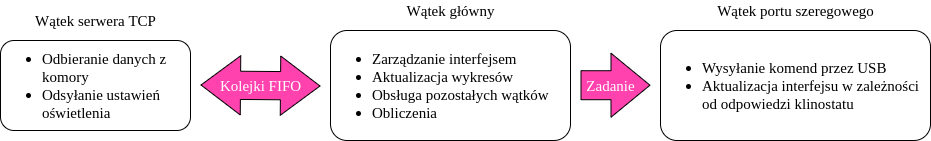
\includegraphics[scale=0.46]{schemat_watki}
	\caption{Schemat budowy wątkowej aplikacji. Źródło: [opracowanie własne]} 
	\label{fig:watki}
	
\end{figure}

\section{Graficzny interfejs użytkownika}

Ten podrozdział poświęcony został opisowemu przedstawieniu graficznego interfejsu użytkownika. Podczas jego tworzenia kierowano się tym, aby był on czytelny oraz intuicyjny w obsłudze. 

\section{Drzewo projektu}

\section{Zabezpieczenia aplikacji}